\section{Evaluation}
\label{sec:Auswertung}

%Siehe \autoref{fig:plot}!
\subsection{LED and Laser}
\label{sec:lec_laser}
In \autoref{subfig:card_led} the diode laser is not lasing.
The threshold for lasing is not reached, so no stimulated emission can take place and the diode laser is acting as an LED.
The \autoref{subfig:card_laser} on the right side shows the laser just above the threshold.
There is a very bright spot at slightly higher voltage.
\begin{figure}
   \caption{Infrared Viewing Card to make the laser beam visible. Photo taken with the CCD-Camera.}
   \begin{subfigure}{0.48\textwidth}
       \centering
       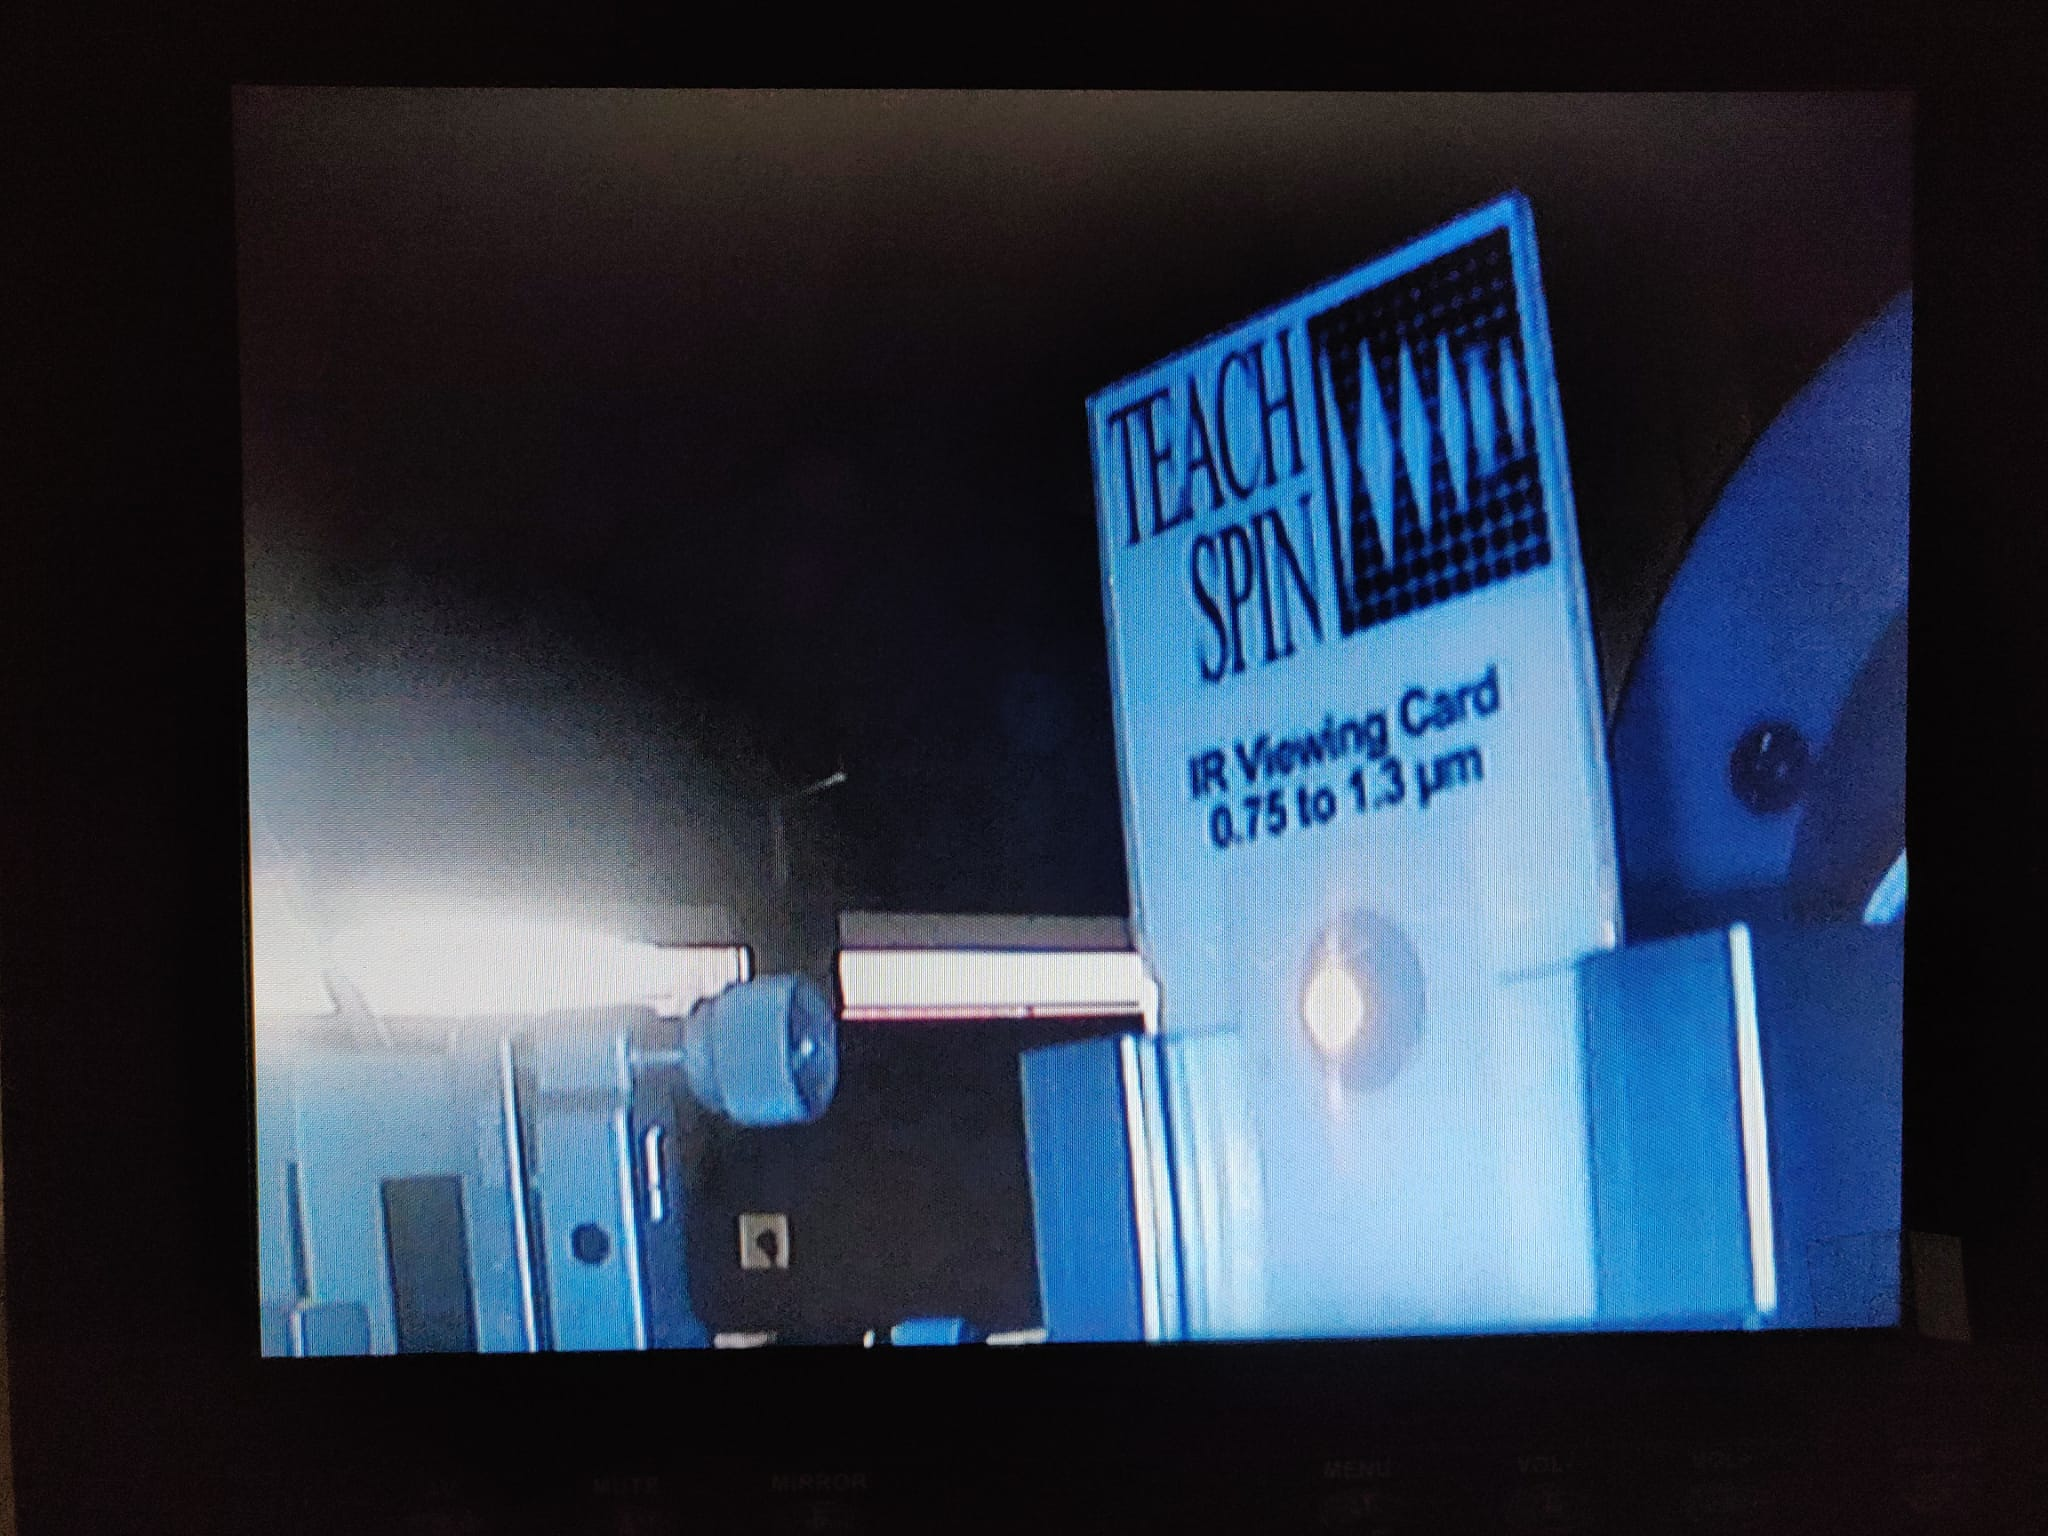
\includegraphics[height=5cm]{content/data/laser_led.jpeg}
       \caption{The laser current is just below the threshold and the laser produces normal light like LEDs.}
       \label{subfig:card_led}
   \end{subfigure}
   \hfill
   \begin{subfigure}{0.48\textwidth}
       \centering
       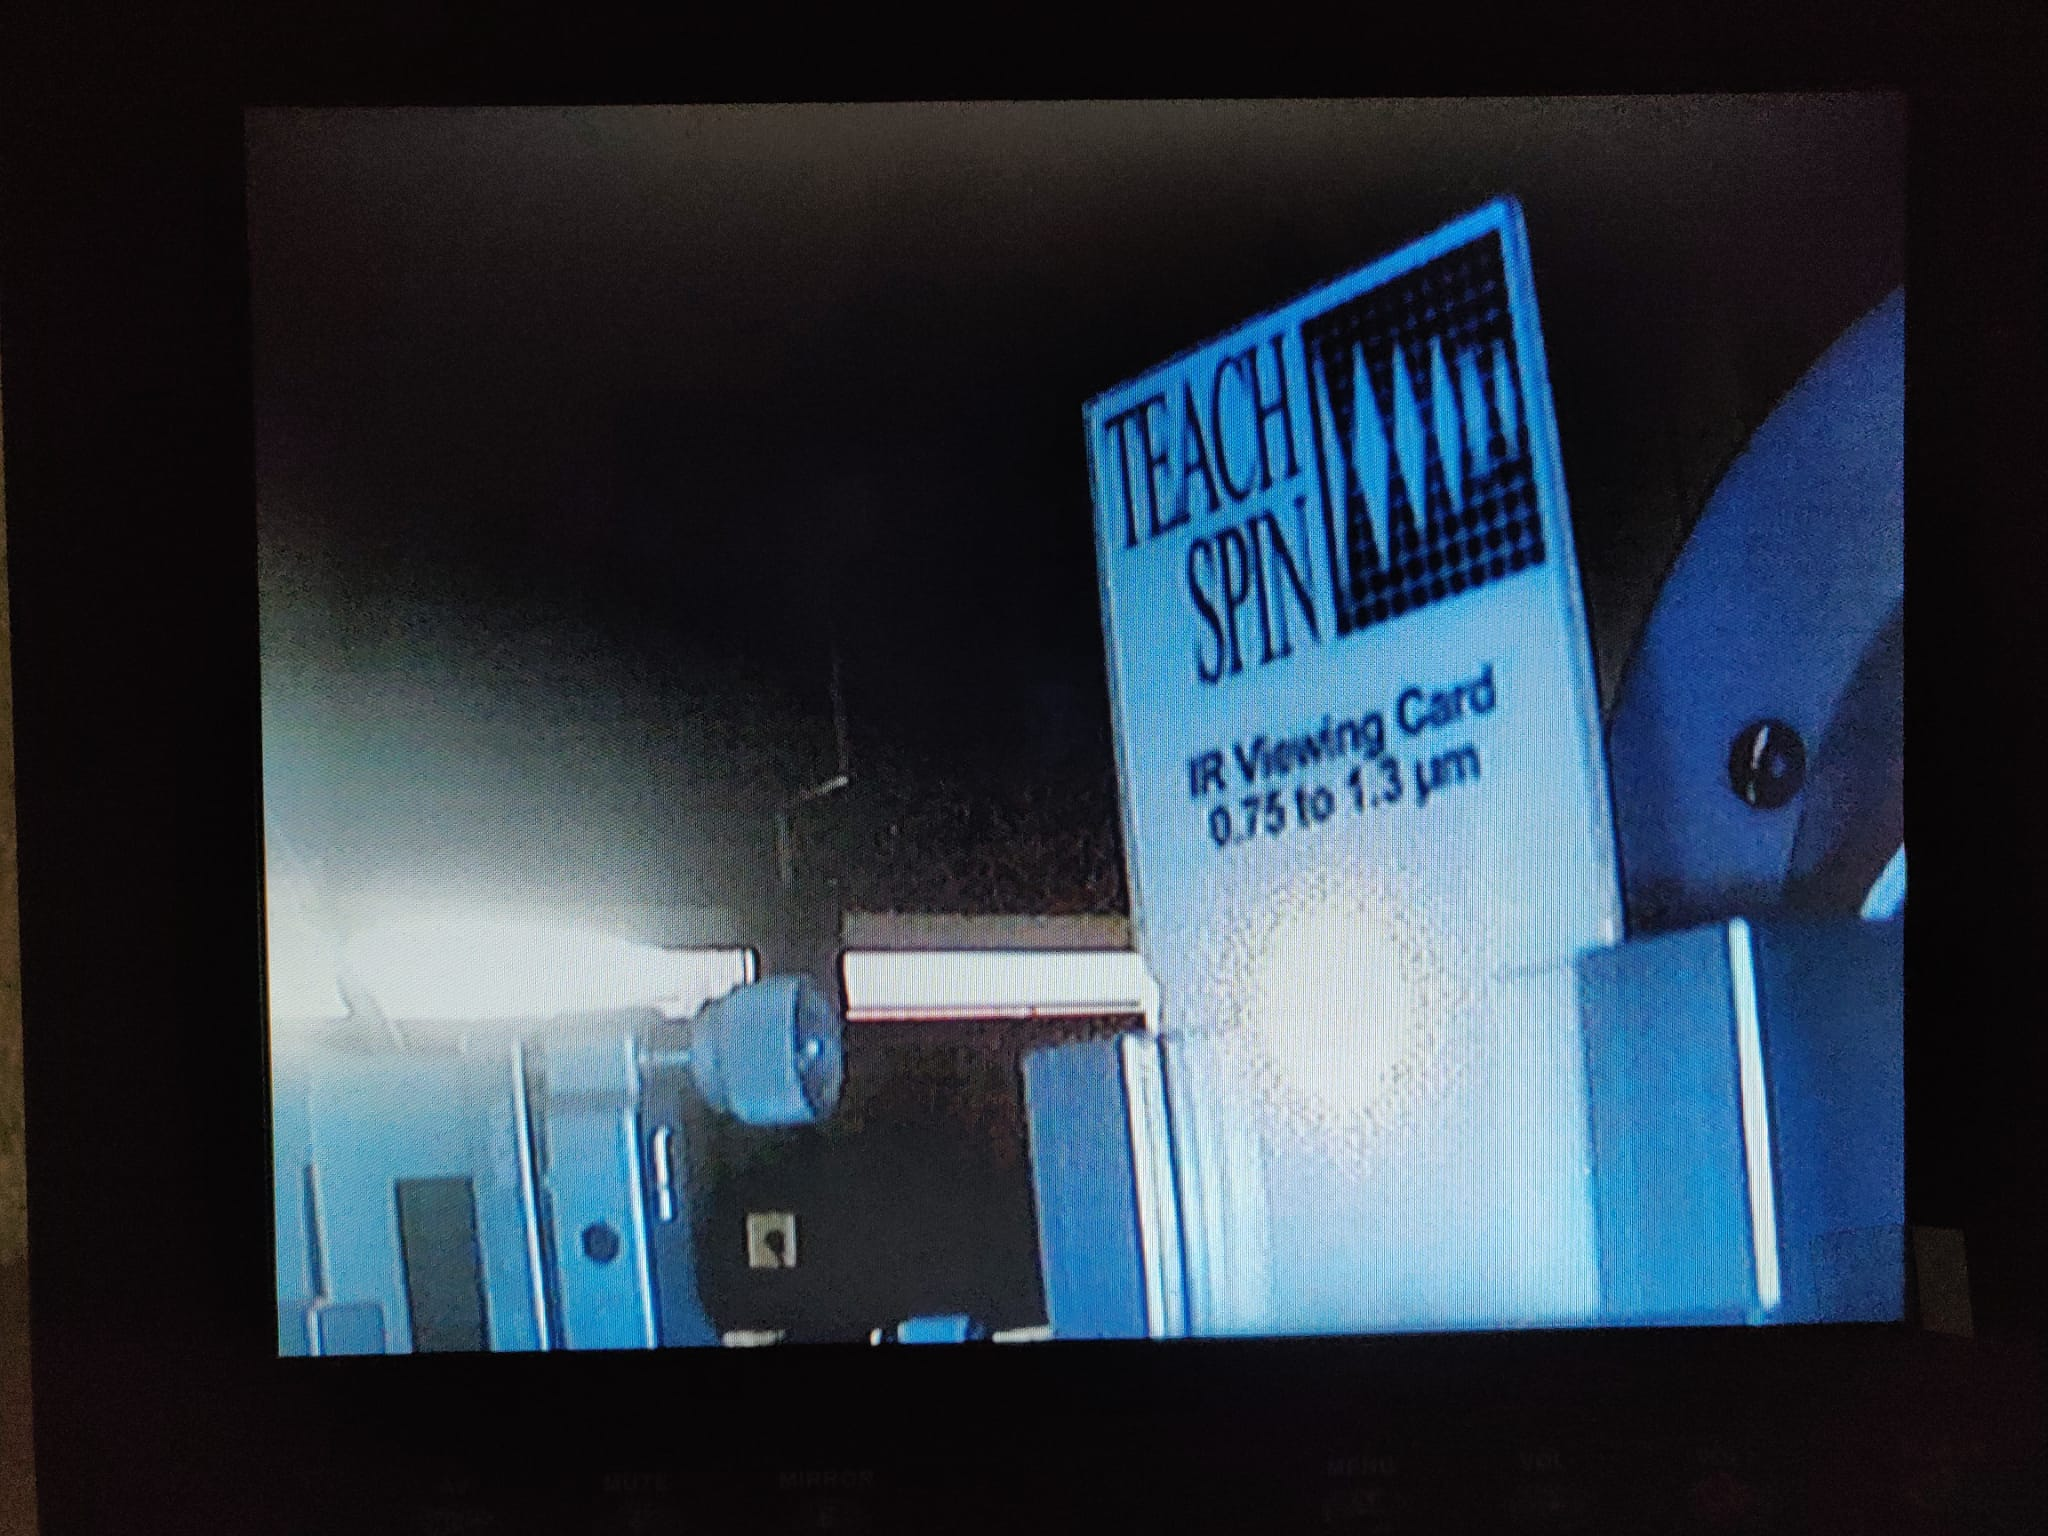
\includegraphics[height=5cm]{content/data/Laser_lasing.jpeg}
       \caption{The laser current just above the threshold.}
       \label{subfig:card_laser}
   \end{subfigure}
   \label{fig:card}
\end{figure}

\FloatBarrier

\subsection{Rubidium flourescence}
\label{sec:rubidium}

In the following part the laser beam hits the Rubidium Absorption Cell as described in \autoref{sec:flourescence}.
The fluorescence can be seen in \autoref{fig:flourescence}.
\begin{figure}
    \centering
    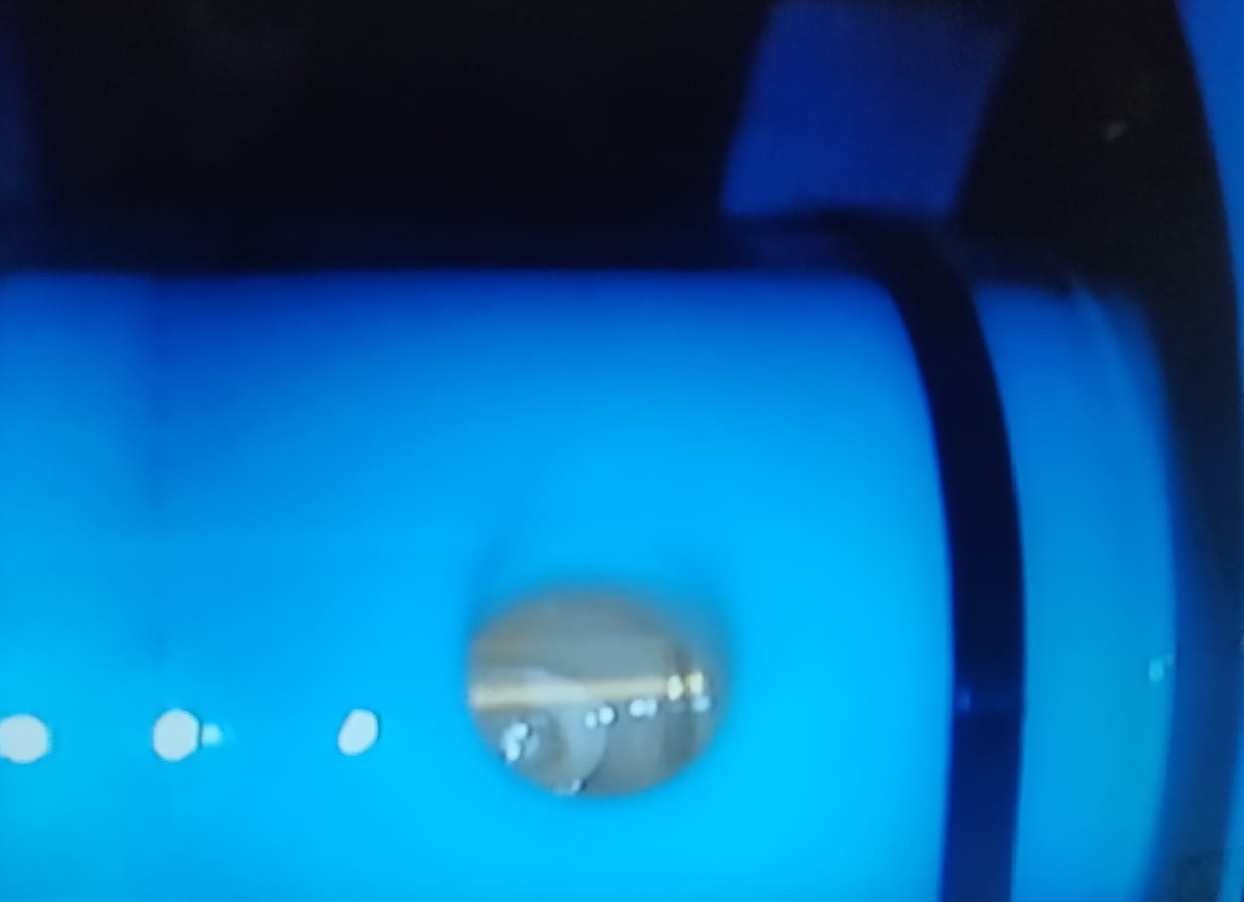
\includegraphics[width=0.6\textwidth]{content/data/flourescence_scaled.jpeg}
    \caption{Rubidium Absorption Cell recorded with the CCD-Camera.}
    \label{fig:flourescence}
\end{figure}
\FloatBarrier

\clearpage
\subsection{Absorption Spectrum of Rubidium}
\label{sec:absorption}

As described in \autoref{sec:absorption_spectrum} the laser beam coming through the Rb cell is now intercepted by a detector.
Also the the undisturbed laser beam hits a further detector.
The difference between the two signals is displayed on the oscilloscope.
After some adjustments the \autoref{fig:absorption_spectrum} was created.
It clearly shows the four absorption lines of $^{85}$Rb and $^{87}$Rb.
\begin{figure}
    \centering
    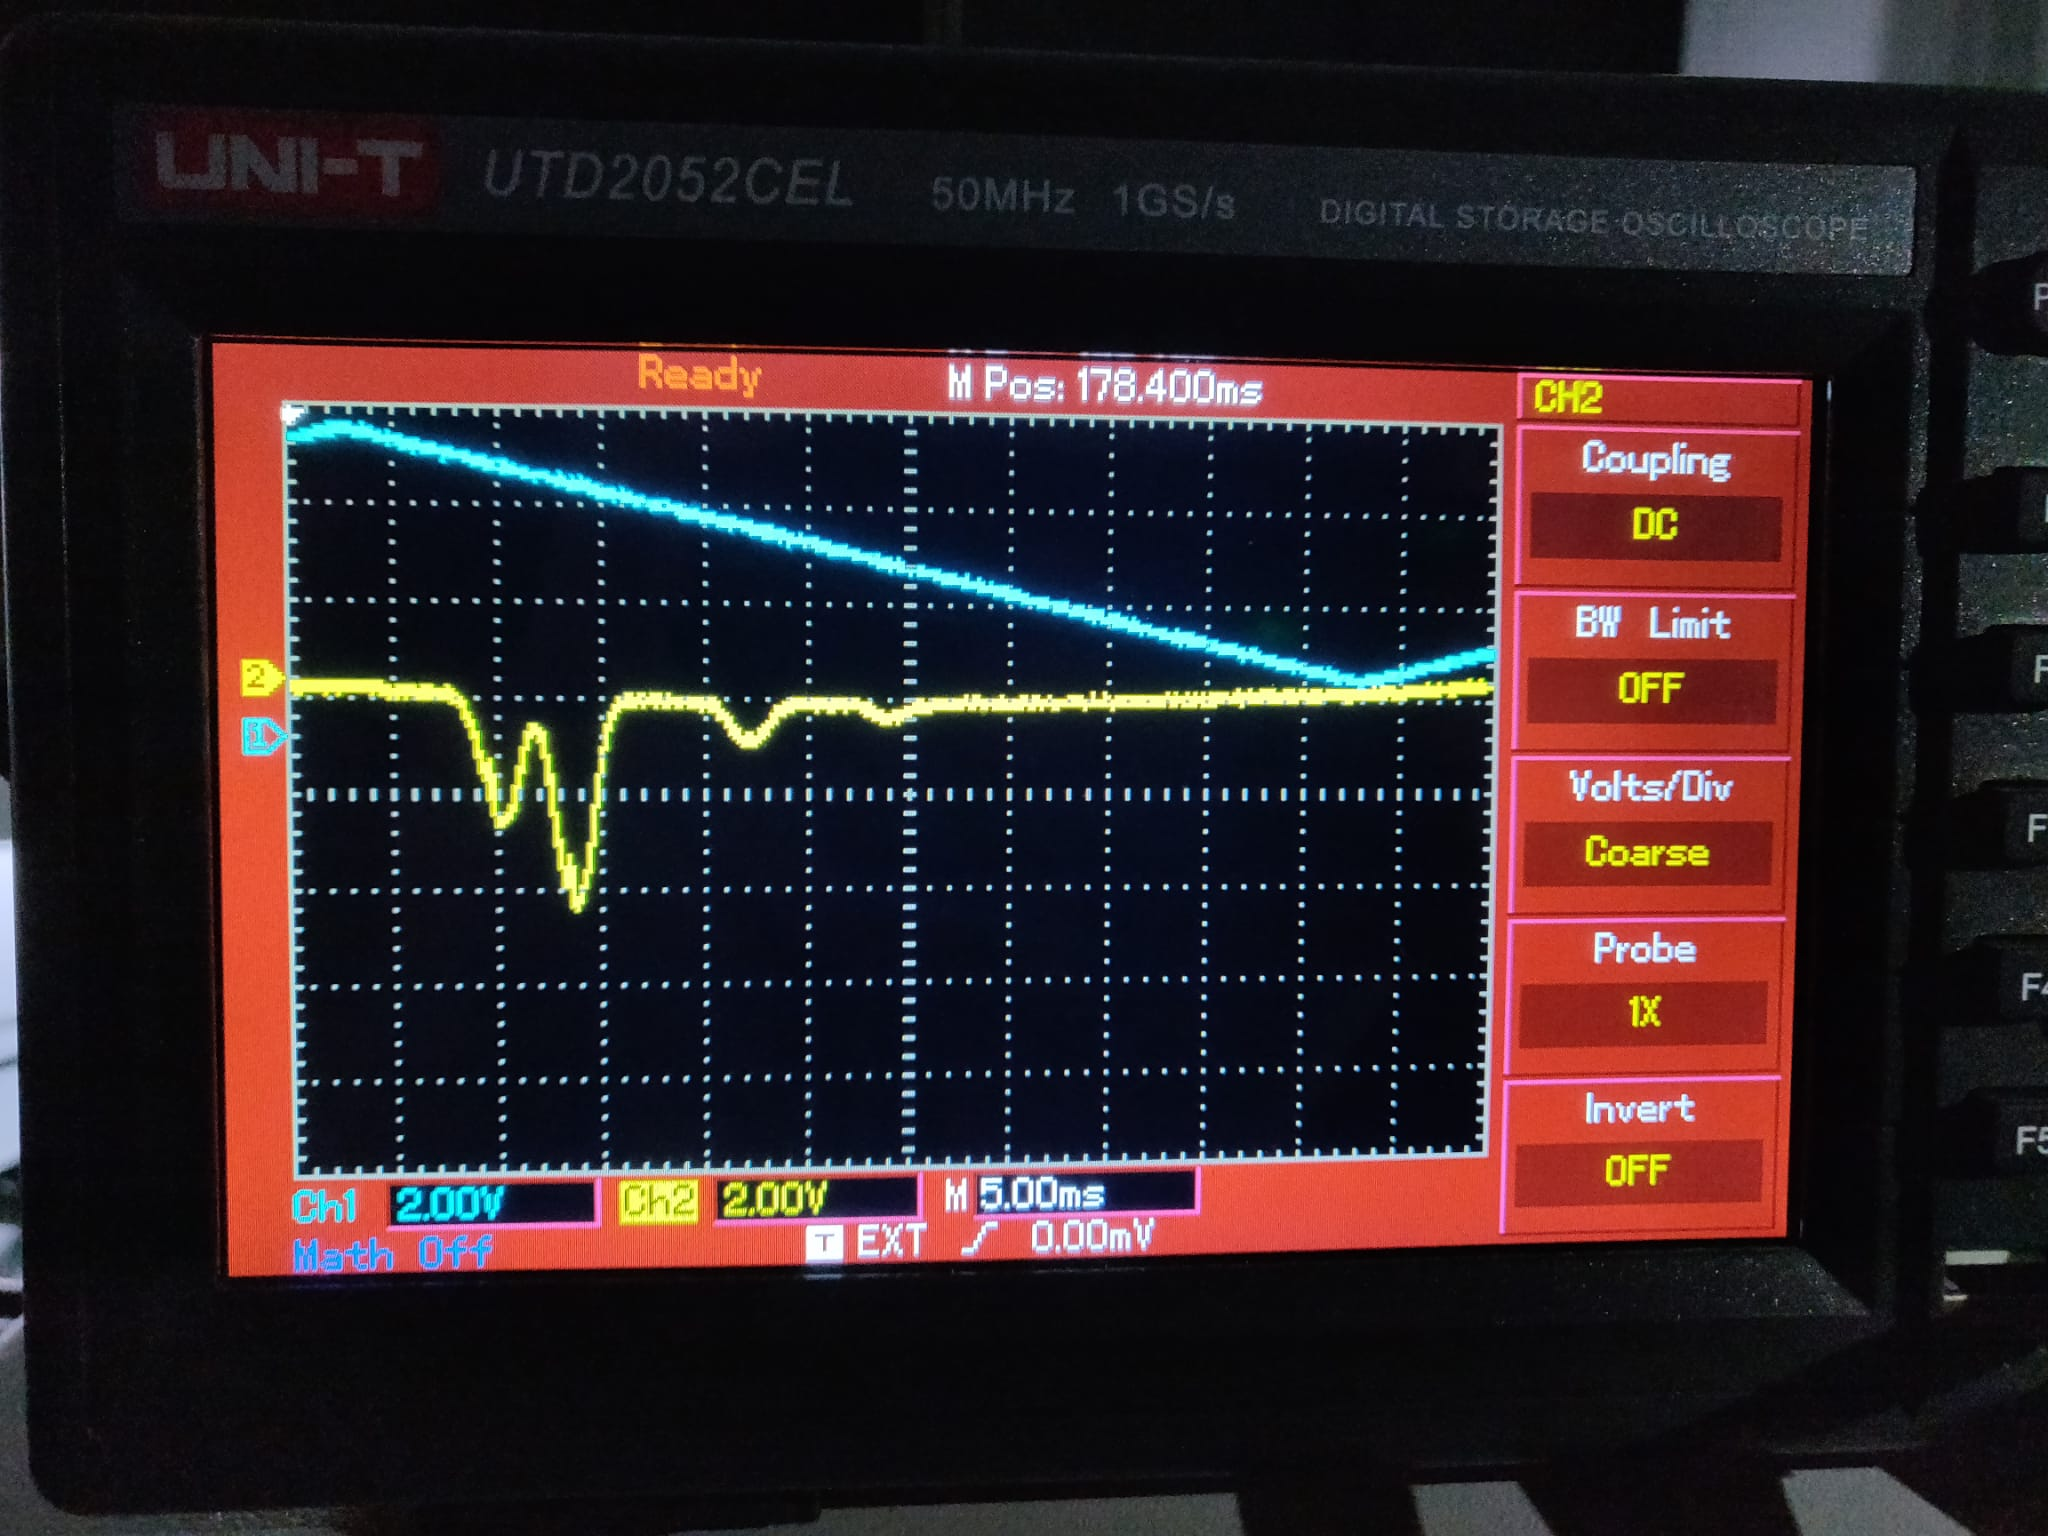
\includegraphics[width=0.8\textwidth]{content/data/Absorption_spectrum.jpeg}
    \caption{Combined signal from the detectors.}
    \label{fig:absorption_spectrum}
\end{figure}